% 全同粒子的统计
% 全同粒子|量子力学|Fork 空间

为什么要讲全同粒子呢?因为,我们的世界有两种粒子,玻色子和费米子,他们的性质截然不同,但又都很重要. 上一章讲了基本的数学结构,这一章就是对这两种粒子建立这种数学结构. 要注意,只有玻色子和费米子这两种粒子在低维的时候很可能被打破,形成一种“任意子(anyon)”,甚为可怕,其在量子信息中也有很重要的作用,是处理非 Abelian 交换的,可做逻辑门. 更多信息可以参考\cite{Nayak2008}.

\subsection{Fock空间}

一个简单的说法,Fock 空间就是不同粒子数的态所在的空间. 例如,一个玻色体系,有两个能级,那么第一个能级 $n$ 个粒子,第二个能级 $m$ 个粒子的态,我们并不关心其具体的波函数形式 $\psi(x)$ 这样的,而是抽象的写成 $|n,m\rangle$. 当然,这里我们还没有明确的定义玻色和费米体系都是什么样子, 这个只是简单的给一个大致想法. 接下来,我们仔细的构建这套理论.

\subsubsection{有关排列群}

首先,我们看一些有关于排列群的知识. 这部分不是必要的,对于理解某些特殊的问题时有奇效\footnote{但是大多数时候这是用来装逼的,不想看的话跳过就可以了}.

\subsubsection{全同粒子的传统处理方法}

如果我有 $n$ 个粒子,由于是全同的,我说这 $n$ 个粒子在 ${\mathrm x}_1, {\mathrm x}_2 \dots {\mathrm x}_n$ 这 $n$ 个位置组成的\textbf{无序数组}的情况可以用类似我们single particle的办法描述,也就是使用波函数
\begin{equation}
\psi({\mathrm x}) = \psi({\mathrm x}_1, {\mathrm x}_2\dots {\mathrm x}_n)
\end{equation}

然而这个波函数的 $n$ 个位置参数显然是有序的. 我们可以断言,在这 $n$ 个坐标进行重新排列之后,波函数应该不变——或者至少说,密度矩阵不变,波函数有相位差别.

在波函数的形式仅仅是一个函数——并不是什么旋量啊之类的奇怪的东西,而仅仅是一个复数的时候(这也被叫做排列群的一维表示),粒子自然而然地被分为了两类:波色子和费米子.

我们取一个排列算符 $\sigma\in S_n$,并将这个算符作用在波函数的参数上,得到的应该是一个对应的一维表示 $R(\sigma)$ 作用在波函数上
\begin{equation}
\psi(\sigma ({\mathrm x}_1, {\mathrm x}_2\dots{\mathrm x}_n)) = R(\sigma)\psi({\mathrm x}_1, {\mathrm x}_2\dots{\mathrm x}_n)
\end{equation}

显然满足的是 $|R(\sigma)| = 1$. 现在考虑一对位置的交换,比如把 $i$ 位置和 $j$ 位置进行交换,这样的操作记为 $\sigma_{i,j}$. 显然的有 $R(\sigma_{i,j})^2 = 1$,也就是说
\begin{equation}
R(\sigma_{i,j}) = \pm 1
\end{equation}

如果更具体的分析这两种群表述的区别,在量子场论里面我们能一目了然的看到这与自旋之间有着密切的关系. 在后面角动量的部分和相对论性量子力学部分我们也会稍微的提及一点. 不过在这里我只给出结论:得到 $+1$ 结果的是玻色子(Boson),两个粒子交换波函数不变;得到 $-1$ 结果的是费米子(Fermion),两个粒子交换波函数变成原来的负数.

然而,如果波函数不是一个数的话,这有可能就是一个排列群的二维或者更复杂的表示了,我们在此不赘述.

\subsubsection{多体 Hilbert 空间的数学结构}

波函数所在的 Hilbert 空间,在这套框架下是没有确定粒子数的空间,也就是说最终的 Hilbert 空间——Fock空间,是各个粒子数的 Hilbert 空间的\textbf{直和}.
\begin{equation}
\mathcal{F} = \mathcal{H}_0 \oplus \mathcal{H}_1\dots
\end{equation}

而我们可以一目了然的说明的就是,$0$ 粒子状态就是一种我们称为“真空”的状态,可以用 $|0\rangle$ 来指代. 更准确一点地说,真空态相当于在 $1$ 粒子波函数的 Hilbert 空间中没有粒子(波函数等于 $0$),而 $1$ 粒子波函数的 Hilbert 空间就是单体波函数所在的线性空间,也是如果我们有一些简单的波动力学基础的话最熟悉的那种.

而更高粒子数的子空间 $\mathcal{H}_n$,则是指通过对称化或者反对称化之后的 $n$ 个单粒子空间的\textbf{张量积的子空间},$(\mathcal{H}_1)^{\otimes n} \equiv \mathcal{H}_1\otimes \mathcal{H}_1\dots\otimes\mathcal{H}_1$,如\autoref{IdParS_fig1} 就是一个张量积的示意.

\begin{figure}[ht]
\centering
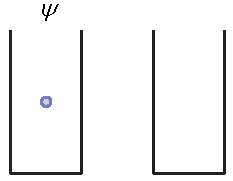
\includegraphics[width=4cm]{./figures/IdParS1.pdf}
\caption{体系的波函数为 $|\psi\rangle_\text{left}\otimes|0\rangle_\text{right}$} \label{IdParS_fig1}
\end{figure}

而我们注意到,$\mathcal{H}_n$ 仅仅是张量积的子空间,要建立完整的数学描述还需要告诉我们如何从这个张量积空间获得这个需要的子空间. 也就是说,形式上的,我们需要找到这么一个线性映射:
\begin{align}
\mathcal{S}:\quad\quad\quad\quad\quad\quad\quad\quad (\mathcal{H}_1)^{\otimes n}&\mapsto\mathcal{H}_n\\
|\psi_1\rangle\otimes|\psi_2\rangle\otimes\dots\otimes|\psi_n\rangle &\mapsto|\psi_1,\psi_2,\dots,\psi_n\rangle
\end{align}

很显然的,我们就得到了两种情况下的这个线性映射 $\mathcal{S}$:
\begin{itemize}
\item Boson Case
\begin{equation}
|\psi_1\rangle\otimes|\psi_2\rangle\otimes\dots\otimes|\psi_n\rangle \mapsto \sum_{{\sigma}\in S_n}|\psi_{\sigma(1)}\rangle\otimes|\psi_{\sigma(2)}\rangle\otimes\dots\otimes|\psi_{\sigma(n)}\rangle
\end{equation}
\item Fermion Case
\begin{equation}
|\psi_1\rangle\otimes|\psi_2\rangle\otimes\dots\otimes|\psi_n\rangle \mapsto \sum_{{\sigma}\in S_n}(-1)^{\sigma}|\psi_{\sigma(1)}\rangle\otimes|\psi_{\sigma(2)}\rangle\otimes\dots\otimes|\psi_{\sigma(n)}\rangle
\end{equation}
\end{itemize}

其中,熟悉线性代数的同学肯定会猜到,这个 $(-1)^{\sigma}$ 就是一个重排操作 $\sigma$ 中交换的次数,或者说逆序数.

接下来我们考虑多体问题 Hilbert 空间的基. 最基础的版本是我们的波函数是空间坐标的函数,当然是多个空间坐标:$\psi(x_1,\dots,x_n)$. 但是,由于统计性质的要求,我们要求(对 Boson 取 $+$,Femrion 取 $-$)
\begin{equation}
\psi(x_1,\dots,x_n)=\frac{1}{\sqrt{n!}}\sum_{\sigma\in S_n}(\pm1)^\sigma\langle x_1|\psi_{\sigma(1)}\rangle\dots\langle x_n|\psi_{\sigma(n)}\rangle
\end{equation}

\begin{exercise}{练习(Majorana 算符)}
考虑两个格点,这两个格点上有相同的费米子模式. 记 $|1\rangle_{1,2}=c_{1,2}\Her|0\rangle$,

(1) 在
\begin{equation}
\left(\begin{matrix}|0\rangle_1|0\rangle_2\\|0\rangle_1|1\rangle_2\\|1\rangle_1|0\rangle_2\\|1\rangle_1|1\rangle_2\end{matrix}\right) 
\end{equation}
的基下,写出 $c_{1,2}, c_{1,2}\Her$ 的矩阵形式. 此处我们定义 $|1\rangle_1|1\rangle_2\equiv c_1\Her c_2\Her|0\rangle_1|0\rangle_2$.
\end{exercise}